\documentclass[oneside, 12pt, a4paper]{article}
\usepackage{amsmath}
\usepackage{graphicx}
\usepackage{fancyhdr}
\usepackage{geometry}
\usepackage{hyperref}
\usepackage{lastpage}
\usepackage{float}
\usepackage{longtable}
\usepackage{booktabs}
%\usepackage[T1]{fontenc}
%\usepackage[utf8]{inputenc}
\usepackage{fontspec}

% Set font
\setmainfont{Arial}



% Load natbib. biber would be preferable, didn't work as expected
\usepackage{natbib}
\bibliographystyle{unsrtnat}

\geometry{a4paper, top = 22mm, left = 25mm, right = 15mm, bottom = 25mm}
\setlength{\headheight}{28pt}



\pagestyle{fancy}
% Create Header for all non-title pages
\fancyhead[L]{
Lorem Ipsum Corp.\\
03/FEB/2021}
\fancyhead[C]{Lorem Ipsum - Report \\}
\fancyhead[R]{
\includegraphics[height=0.75cm]{gpc-service-logo.png}
}

% Create footer with document meta data
\fancyfoot[R]{Page \thepage\phantom{ }of \pageref*{LastPage}}
\fancyfoot[L]{template\_name\_D01}
\fancyfoot[C]{Effective Date: 01/JAN/1960}

\begin{document}
\begin{titlepage}
   \begin{center}
    
\includegraphics[width=0.6\textwidth]{gpc-service-logo.png}
       \vspace*{1cm}
        \vfill
        \huge
        \textbf{Lorem Ipsum - Report} \\
        \large
        \vspace{0.5cm}
        enter subtitle or leave blank\\
        \vspace{0.5cm}
        Date: 03/FEB/2021\\
        \vspace{1.5cm}
        \vfill
        \vspace{0.8cm}

\begin{flushleft}
Ronald A. Fisher\\
GCP-Service International Ltd. \& Co. KG \\
Anne-Conway-Str. 2 \\
28359 Bremen, Germany \\
E-mail: \href{mailto:rfisher@gcp-service.com}{\nolinkurl{rfisher@gcp-service.com}}\\
Tel +49 (0)421 20 80 98 51
\end{flushleft}
\end{center}

\end{titlepage}

% Add ToC
\tableofcontents
\newpage
\listoffigures
\newpage
\listoftables
\newpage
% Start of actual document

% body will be replaced by the text that is compiled in the *.rmd file
\hypertarget{this-section-title-is-created-using-rmd-syntax}{%
\section{This Section Title is created using
rmd-syntax}\label{this-section-title-is-created-using-rmd-syntax}}

The following text is filler and can be replaced by real content. I
really recommend having a look at the rmarkdown cheat sheet:
\url{https://rstudio.com/wp-content/uploads/2015/02/rmarkdown-cheatsheet.pdf}
The next is created using LateX!

\hypertarget{text}{%
\section{Text}\label{text}}

\hypertarget{basic-text}{%
\subsection{Basic Text}\label{basic-text}}

Lorem ipsum dolor sit amet, consetetur sadipscing elitr, sed diam nonumy
eirmod tempor invidunt ut labore et dolore magna aliquyam erat, sed diam
voluptua. At vero eos et accusam et justo duo dolores et ea rebum. Stet
clita kasd gubergren, no sea takimata sanctus est Lorem ipsum dolor sit
amet. Lorem ipsum dolor sit amet, consetetur sadipscing elitr, sed diam
nonumy eirmod tempor invidunt ut labore et dolore magna aliquyam erat,
sed diam voluptua. At vero eos et accusam et justo duo dolores et ea
rebum. Stet clita kasd gubergren, no sea takimata sanctus est Lorem
ipsum dolor sit amet.

Section headers can be written after a number of pound signs, e.g.,

\begin{verbatim}
# First-level header

## Second-level header

### Third-level header
\end{verbatim}

\hypertarget{quoting-text}{%
\subsection{Quoting text}\label{quoting-text}}

\begin{verbatim}
> "This is quoted text."
>
> --- Autor
\end{verbatim}

\begin{quote}
``This is quoted text.''

--- Autor
\end{quote}

\hypertarget{math-expressions}{%
\subsection{Math expressions}\label{math-expressions}}

\hypertarget{using-alignment}{%
\subsubsection{Using alignment}\label{using-alignment}}

Here is a model:

\begin{align}
Y = \beta_0 + \beta_1 X_i + \epsilon \\
Y_i = \beta_0 + \beta_1 X_i + \epsilon_i ,
\end{align} and here is some unnumbered equation: \begin{align*}
a^2 + b^2 = c^2
\end{align*}

\hypertarget{alternative}{%
\subsubsection{Alternative}\label{alternative}}

Math expressions of the display style can be written in a pair of double
dollar signs, e.g

\[{\displaystyle f_{Y}(\mathbf {y} \mid {\boldsymbol {\theta }},\tau )=h(\mathbf {y} ,\tau )\exp \left({\frac {\mathbf {b} ({\boldsymbol {\theta }})^{\rm {T}}\mathbf {T} (\mathbf {y} )-A({\boldsymbol {\theta }})}{d(\tau )}}\right).\,\!}\]

Inline LaTeX equations can be written in a pair of dollar signs using
the LaTeX syntax,
e.g.~\({\displaystyle f_{Y}(\mathbf {y} \mid {\boldsymbol {\theta }},\tau )}\)

\hypertarget{codes}{%
\subsection{Codes}\label{codes}}

Sometimes you may need some SAS code

\begin{verbatim}
proc univariate data = whas500(where=(fstat=1));
  var lenfol;
  histogram lenfol / kernel;
run;
\end{verbatim}

\hypertarget{plot}{%
\section{Plot}\label{plot}}

\hypertarget{insert-r-plots}{%
\subsection{Insert R Plots}\label{insert-r-plots}}

Here are some nomally distributed random numbers:

\begin{figure}[H]

{\centering 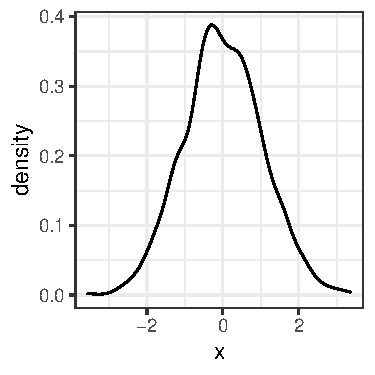
\includegraphics{C:/Users/zbai/Desktop/Untitled/report_files/figure-latex/normal_plot-1} 

}

\caption{\label{fig:fig1}Density of normally distributed random numbers.}\label{fig:normal_plot}
\end{figure}

Here is an overview of \(\chi^2\)-distributions with various degrees of
freedom:

\begin{figure}[H]

{\centering 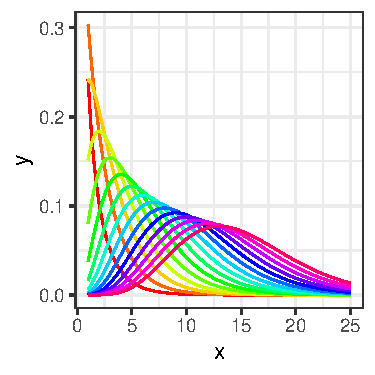
\includegraphics{C:/Users/zbai/Desktop/Untitled/report_files/figure-latex/chisq_plot-1} 

}

\caption{\label{fig:fig2}$\chi^2$-distributions.}\label{fig:chisq_plot}
\end{figure}

This is the end of this section. Have some references to the plots
before you leave (see figs. \ref{fig:fig1} and \ref{fig:fig2}).

\hypertarget{insert-external-figures}{%
\subsection{Insert external figures}\label{insert-external-figures}}

Insert one external figure:

\begin{center}

\includegraphics[width=3.5 in]{Z:/STATISTICS/08_Team/RPA/GCPS2021/inst/rmarkdown/templates/gcps2021/skeleton/gpc-service-logo.png}
\begin{figure}[!h]
\caption{This is the figure caption}
\end{figure}
\end{center}

\hypertarget{table}{%
\section{Table}\label{table}}

\hypertarget{create-a-r-table}{%
\subsection{Create a R Table}\label{create-a-r-table}}

\begin{longtable}[]{@{}lrrrrr@{}}
\caption{Summary of Edgar Anderson's Iris Data}\tabularnewline
\toprule
& Sepal.Length & Sepal.Width & Petal.Length & Petal.Width &
Species\tabularnewline
\midrule
\endfirsthead
\toprule
& Sepal.Length & Sepal.Width & Petal.Length & Petal.Width &
Species\tabularnewline
\midrule
\endhead
Min. & 4.300000 & 2.000000 & 1.000 & 0.100000 & 50\tabularnewline
1st Qu. & 5.100000 & 2.800000 & 1.600 & 0.300000 & 50\tabularnewline
Median & 5.800000 & 3.000000 & 4.350 & 1.300000 & 50\tabularnewline
Mean & 5.843333 & 3.057333 & 3.758 & 1.199333 & 50\tabularnewline
3rd Qu. & 6.400000 & 3.300000 & 5.100 & 1.800000 & 50\tabularnewline
Max. & 7.900000 & 4.400000 & 6.900 & 2.500000 & 50\tabularnewline
\bottomrule
\end{longtable}

The R extension package pander provides better table capabilities and
can also work well with the knitr package for output. Its pander()
function can convert a variety of R output formats into the table form
required by knitr.

\hypertarget{create-custom-tables}{%
\subsection{Create custom tables}\label{create-custom-tables}}

\begin{longtable}[]{@{}lll@{}}
\caption{\centering This is the table caption (left
alignment)}\tabularnewline
\toprule
Colname 1 & Colname 2 & \ldots{}\tabularnewline
\midrule
\endfirsthead
\toprule
Colname 1 & Colname 2 & \ldots{}\tabularnewline
\midrule
\endhead
AAA & \ldots{} & \ldots{}\tabularnewline
AAAA & \ldots{} & \ldots{}\tabularnewline
AAAAA & \ldots{} & \ldots{}\tabularnewline
\bottomrule
\end{longtable}

\begin{longtable}[]{@{}ccc@{}}
\caption{\centering This is the table caption (center
alignment)}\tabularnewline
\toprule
Colname 1 & Colname 2 & \ldots{}\tabularnewline
\midrule
\endfirsthead
\toprule
Colname 1 & Colname 2 & \ldots{}\tabularnewline
\midrule
\endhead
AAA & \ldots{} & \ldots{}\tabularnewline
AAAA & \ldots{} & \ldots{}\tabularnewline
AAAAA & \ldots{} & \ldots{}\tabularnewline
\bottomrule
\end{longtable}

\begin{longtable}[]{@{}rrr@{}}
\caption{\centering This is the table caption (right
alignment)}\tabularnewline
\toprule
Colname 1 & Colname 2 & \ldots{}\tabularnewline
\midrule
\endfirsthead
\toprule
Colname 1 & Colname 2 & \ldots{}\tabularnewline
\midrule
\endhead
AAA & \ldots{} & \ldots{}\tabularnewline
AAAA & \ldots{} & \ldots{}\tabularnewline
AAAAA & \ldots{} & \ldots{}\tabularnewline
\bottomrule
\end{longtable}

\hypertarget{conclusion}{%
\section{Conclusion}\label{conclusion}}

This is a nice template, says \cite{fisher_statistical_1970} (acutally,
he doesn't. I just wanted to show one possible way of adding
literature).

\newpage
\addcontentsline{toc}{section}{References}
%\addcontentsline{toc}{chapter}{References}
\bibliography{references}
\end{document}
